\documentclass[a4paper]{article}
%define coloursIn Section 4 the conclusions from this experiment are summarised, and possible avenues for further experimentation are briefly explored.
\usepackage{xcolor}
\usepackage{sectsty}
\definecolor{purply}{HTML}{055c5b}
\definecolor{gurple}{HTML}{055c5b}
%%maths stuff
\usepackage[]{amsmath}
\usepackage{amssymb}
\usepackage{url}
\usepackage{cancel}
%%pictures
\usepackage{graphicx}
\usepackage{subcaption}
\graphicspath{{./pics/}}
%%pagestyle
\usepackage[margin=1in]{geometry}
\usepackage[shortlabels]{enumitem}
\usepackage{fancyhdr}
\pagestyle{fancy}
\fancyhf{}
\fancyfoot[R]{\color{gurple} Page \thepage}
\renewcommand{\sectionmark}[1]{\markright{#1}}
\fancyhead[L]{\color{gurple} \nouppercase{\rightmark}}
%\lhead{\color{gurple} NP08 - Lifetime of the Muon \rightmark}
%\rfoot{\color{gurple} Page \thepage}
\sectionfont{\color{purply}}
%%code
\usepackage{listings}
\lstset{frame=tb,
	%style=Matlab-editor,
	aboveskip=3mm,
	belowskip=3mm,
	showstringspaces=false,
	columns=flexible,
	basicstyle={\small\ttfamily},
	numbers=none,
	breaklines=true,
	breakatwhitespace=true,
	tabsize=3
}
%citations
\usepackage[backend=biber,citestyle=authoryear,bibstyle=numeric,firstinits=true,autocite=footnote]{biblatex}
\addbibresource{ref.bib}
%\usepackage[nottoc,notlot,notlof]{tocbibind}
\usepackage[nottoc,notlot,notlof,numbib]{tocbibind}
%%final styling

\usepackage{pgfplots}
\usepackage{tikz}
\pgfplotsset{compat=1.15}
\usepackage{mathrsfs}
\usetikzlibrary{arrows}

\usepackage[charter]{mathdesign}
\title{\color{purply} \Huge NP08 Miniproject: Lifetime of the Muon}
\author{\LARGE  Zella Baig\\
shil5321}
\def\muu{\ensuremath\mu\ }
\begin{document}
\maketitle
\thispagestyle{empty}
\begin{abstract}
	\noindent In
	this experiment we examine the lifetime of the muon using a series of scintillators connected to photomultiplier tubes, in order to determine stopping events which produce electrons. We perform a series of selection cuts on the dataset to isolate desired signals from background noise, and determine the lifetime of the muon to be $\tau = (2.57 \pm 0.41) \times 10^{-6}$s, a range encompassing the commonly accepted value of $\tau_\mu = 2.20 \times 10^{-6}$s. Further, we explore the number of concurrent (i.e. from the same source) events we are able to view employing a secondary scintillator, which we are able to move further away from the main apparatus. We determine, as expected, that as distance is increased the number of events seen is reduced (due to the same number of events needing to cover a wider solid angle projected from the creation event); given the limited number of trials we are able to perform with this aspect of the experiment we cannot yet claim any quantitative relationship.
\end{abstract}
\newpage
\tableofcontents
\thispagestyle{empty}
\newpage
\setcounter{page}{1}
\section{Introduction}
The muon ($\mu$) is a $2^{nd}$ generation lepton, similar to the electron although more massive at $105.66$ MeV/c$^2$ (or $206.77 m_e$)\footcite{muonmass}. The muon undergoes decays of the form:
\begin{equation*}
	\mu \rightarrow \nu_\mu +e+ \bar \nu_e
\end{equation*}
with a lifetime $\tau_\mu$ of $2.197 \times 10^{-6}$s.
Muons are produced in the upper atmosphere as a result of cosmic ray interactions, which produce pions ($\pi$) that predominantly then decay in the following ways, with the superscripts $+$ and $-$ denoting positively and negatively charged particles, respectively:
\begin{align*}
	&\pi^- \rightarrow \mu^- +\bar \nu_\mu & 
	\pi^+ \rightarrow \mu^+ +\nu_\mu.& 
\end{align*}
The principle of the main aspect of the experiment is to investigate the lifetime of the muon, from observing the decays in four different scintillators (denoted $A,B,C,D$), as shown in Figure 1:
%%%% TIKZ
\begin{figure}[h!]
\begin{center}
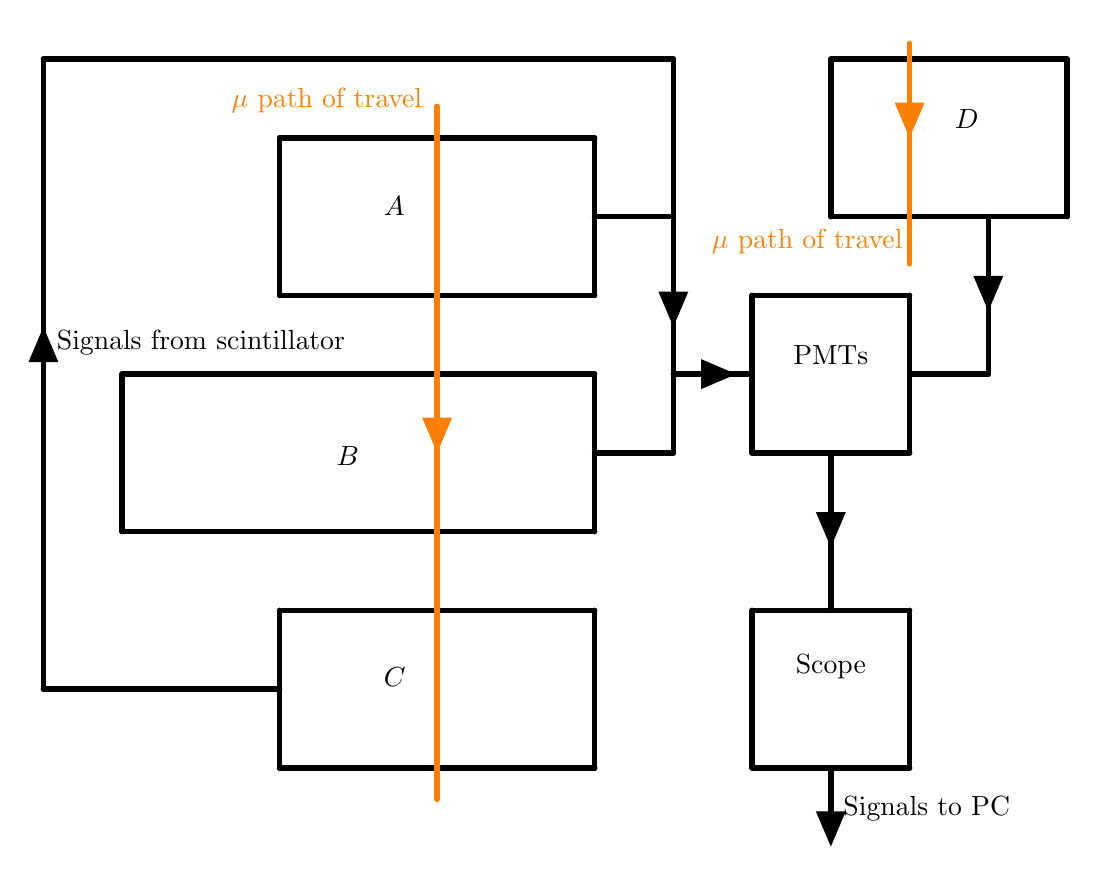
\begin{tikzpicture}[line cap=round,line join=round,>=triangle 45,x=1cm,y=1cm]
\begin{axis}[
x=2cm,y=2cm,
axis lines=middle,
ymajorgrids=false,
xmajorgrids=false,
axis line style={draw=none},
ticks=none,
xmin=-3.6,
xmax=3.1,
ymin=-2,
ymax=3.2]
\clip(-4,-2) rectangle (3.882222222222227,3.914444444444431);
\draw [->,line width=2pt] (1.5,-1.5)-- (1.5,-2);
\draw [line width=2pt] (2,-0.5)-- (2,-1.5);
\draw [line width=2pt] (1,-1.5)-- (2,-1.5);
\draw [line width=2pt] (1,-0.5)-- (2,-0.5);
\draw [line width=2pt] (1,-0.5)-- (1,-1.5);
\draw [->,line width=2pt] (1.5,0.5)-- (1.5,-0.1);
\draw [line width=2pt] (1.5,0)-- (1.5,-0.5);
\draw [line width=2pt] (1.5,2)-- (3,2);
\draw [line width=2pt] (1.5,2)-- (1.5,3);
\draw [line width=2pt] (3,2)-- (3,3);
\draw [line width=2pt] (1.5,3)-- (3,3);

\draw [->,line width=2pt] (2.5,2)-- (2.5,1.4);
\draw [line width=2pt] (2.5,1.5)-- (2.5,1);

\draw [line width=2pt] (2,1)-- (2.5,1);
\draw [line width=2pt] (-3,0)-- (0,0);
\draw [line width=2pt] (0,1)-- (-3,1);
\draw [->,line width=2pt] (0.5,1)-- (0.9,1);
\draw [,line width=2pt] (0.6,1)-- (1,1);
\draw [line width=2pt] (-3,0)-- (-3,1);
\draw [line width=2pt] (1,0.5)-- (1,1.5);
\draw [line width=2pt] (1,0.5)-- (2,0.5);
\draw [line width=2pt] (2,0.5)-- (2,1.5);
\draw [line width=2pt] (1,1.5)-- (2,1.5);
\draw [line width=2pt] (0,-0.5)-- (0,-1.5);
\draw [line width=2pt] (0,-1.5)-- (-2,-1.5);
\draw [line width=2pt] (-2,-1.5)-- (-2,-0.5);
\draw [line width=2pt] (-2,-0.5)-- (0,-0.5);
\draw [line width=2pt] (-2,-1.5)-- (0,-1.5);
\draw [line width=2pt] (-2,-1)-- (-3.5,-1);
\draw [line width=2pt] (0,1)-- (0,0);
\draw [line width=2pt] (0,1.5)-- (-2,1.5);
\draw [line width=2pt] (-2,2.5)-- (-2,1.5);
\draw [line width=2pt] (-2,2.5)-- (0,2.5);
\draw [line width=2pt] (0,2.5)-- (0,1.5);
\draw [line width=2pt] (0,2)-- (0.5,2);
\draw [line width=2pt] (0,0.5)-- (0.5,0.5);

\draw [->,line width=2pt] (0.5,2)-- (0.5,1.3);
\draw [line width=2pt] (0.5,1.8)-- (0.5,0.5);

\draw [line width=2pt] (0.5,2)-- (0.5,3);
\draw [line width=2pt] (0.5,3)-- (-3.5,3);
\draw [->,line width=2pt] (-3.5,-1)-- (-3.5,1.3);
\draw [line width=2pt] (-3.5,1.2)-- (-3.5,3);
\draw [->,line width=2pt,color=orange] (-1,2.7) -- (-1,0.5);
\draw [line width=2pt,color=orange] (-1,0.6) -- (-1,-1.7);
\draw [->,line width=2pt,color=orange] (2,3.1) -- (2,2.5);
\draw [line width=2pt,color=orange] (2,2.6) -- (2,1.7);
\draw (-1.4,2.19) node[anchor=north west] {$A$};
\draw (-1.7,0.6) node[anchor=north west] {$B$};
\draw (-1.4,-0.8) node[anchor=north west] {$C$};
\draw (2.5,2.5) node[anchor=south east] {$D$};
\draw (2.7,-1.9) node[anchor=south east] {Signals to PC};
\draw (1.5,1) node[anchor=south] {PMTs};
\draw (1.5,-1) node[anchor=south] {Scope};
\draw[color=orange] (-1.7,2.6) node[anchor=south] {$\mu$ path of travel};
\draw[color=orange] (1.35,1.7) node[anchor=south] {$\mu$ path of travel};
\begin{scriptsize}
	\draw[color=black] (-2.5,1.2) node {Signals from scintillator};
\end{scriptsize}
\end{axis}
\end{tikzpicture}
\end{center}
\caption{A diagram of the experimental setup, showing scintillators $A$, $B$, $C$, and $D$; the connected photomultiplier tubes (PMTs); and the subsequently connected oscilloscope which feeds into a computer. The path of the muons is shown in orange; scintillators $A$, $B$, and $C$ are stacked on top of one another and so muons interact with them sequentially.}
\end{figure}
\\ \noindent
We denote the sequentially stacked scintillators (i.e. scintillators $A,B,C$) the ``primary'' setup, and ensure the fourth scintillator $D$ is mobile.
Scintillator $D$ is used to investigate concurrent source events across various distances; that is to say, to look for signals detected both in the primary setup and in $D$ such that we can say the source event for both signals was the same.
We use $D$ to investigate the relationship between the distance $X$ of $D$ from the primary setup, and number of concurrent events. We expect as $X$ increases, the number of concurrent events should fall.
This is due to the fact that we can model muon showers to create the same solid angle of projected events onto the surface of the Earth, and so events that are created higher in the atmosphere will be spread over a much larger area by the time they hit the ground and therefore have a lower density of events per square metre. 
\newpage \noindent
The signals from these scintillators are magnified via the PMTs and are then sent to an oscilloscope where we can observe pulses rising above background signals. When examining the muon decays, we expect to observe 2 main types of events: 
\begin{enumerate}
	\item Those in which muons pass straight through all three detectors, giving signals in $A$, $B$, and $C$;
	\item Events in which muons stop in $B$, giving a signal in $A$ and $B$, but none in $C$\footnote{Scintillator $B$ is the thickest of the scintillators, and so we expect a higher likelihood of stopping events to be seen in the form of $B$ signals.}.
\end{enumerate}
\noindent All events leading to pulses in the oscilloscope were registered over a set time period.
Once the events are captured, over a long enough time frame (such that we have enough events to generate statistical uncertainties on our data) we can then ascertain a value for the lifetime of the muon by examining the time delay between secondary pulses in the $B$ scintillator (caused by a muon stopping and decaying into an electron) and the initial signal caused by the muon entering $B$, then examining the time distribution of the decays. 
An exponential curve can be fitted to this distribution of the form 
\begin{equation}
	A\exp \left( \frac{-t}{\tau}  \right),
\end{equation}
to determine our experumental value for the lifetime $\tau$ of the muon, and compare it to the experimental value $\tau_\mu$ as given in the literature\footcite{muonlifetime}.
\\\\
In this experiment, two different extensions were explored. The first of these was to examine the uncertainties arising from the \textit{``cuts''} chosen on the data (the time-based and pulse height-based selection and exclusion of certain events to separate the muon-based signals from background noise), again in order to separate desired signals from background events.
\\\\
The second arose from unexpected behaviour when examining the signals from the scintillators. An unexpected initial peak was observed that caused selected events to resemble a bimodal distribution in their time distribution. The timings of these events were far too quick to be caused by any afterpulses from apparatus effects (which had been considered) and as such, this effect was examined further as to try and determine the cause.
\\\\
Subsequently, in Section 2, we discuss the methodology in detail, drawing particular attention to the ``cuts'' applied and the rationale behind the various cuts used, and the effects to the dataset induced by the cuts themselves. We also discuss in detail the extraction of the lifetime of the muon from the decay time distribution, and present the methods used to examine the bimodal signal peaks. In Section 3 we present an analysis of our results, and examine the statistical uncertainties which arose via our methodology. We end with Section 4, where the conclusions from this experiment are summarised, and possible avenues for further experimentation are briefly explored.
\newpage
\section{Methodology}%

In the setup described in Figure 1, detector $B$ is the thickest scintillator and so we expect the greatest number of muon collision events to be seen from signals originating from it (in comparison to $A$ or $C$).
Importantly, when magnifying the signals from the scintillators via the PMTs, we produce ``afterpulses'' some amount of time later, due to the production of unwanted signals by the production of excited ions within the PMT.
These afterpulses then induce a secondary signal at the cathode - which the oscilloscope will pick up.
This secondary signal is of a lower pulse height than the initial signal, given the lower energy transferred from the ions travelling back to the cathode.
Of course, the travel time of these ions also induces a lag between any initial signals and the afterpulses, which must be accounted for when performing any analysis on the datasets.
\\\\
The data from the oscilloscope was collected in 8ns bins (we use the word ``tick'' to describe such an 8ns interval), with a trigger threshold of -67mV (corresponding to $-1,000$ ADC units; a conversion factor inherent to the hardware \footcite{script}) on the $B$ scope.
This value was determined experimentally after observing the heights of the signals from $B$ manually and adjusting the oscilloscope trigger threshold until a suitable parameter was found.
As the primary setup utilises a different set of PMTs to $D$, a trigger threshold for the latter was found experimentally to be about -30mV; the difference in values arises due to the different parameters of the PMTs corresponding to $B$ and $D$ respectively.
\\\\
The datasets were collected and the previously mentioned ``cuts'' applied, utilising the Pandas\footcite{pandas} framework. We use the naming scheme DF{\bf X}Cut{\bf N} (\textit{DataFrame\footcite{dataframe} \textbf{X}, Cut \textbf{N}}), where $ \textbf{X}$ takes the values:
\begin{itemize}
	\item \textbf{T} = Going through events;
	\item \textbf{S} = Stopping events;
	\item \textbf{U} = Uncorrelated events;
	\item \textbf{All} = Both stopping and throughgoing events;
	\item \textbf{D} = Events in which we examine some $D$ signal;
\end{itemize}
and $N$ represents the cut number.
\\\\
There were 6 initial cuts made for the experiment, denoted Cut1, Cut2, etc.
Note also that unless explicitly stated otherwise, each cut is applied sequentially to whichever dataset it pertains to - e.g. for stopping events, Cut6 is applied directly after Cut5.
The cuts are defined as follows in Table 1:
\begin{table}[h!]
\centering
\begin{tabular}{l|l}
Cut  &  Description\\ \hline
Cut1 & \begin{tabular}[c]{@{}l@{}}
A trigger threshold on the magnitude of a $B$ pulse is required.\end{tabular}\\\\
Cut2 & \begin{tabular}[c]{@{}l@{}}$A$ events are required to be within a 20$\mu s$ window (i.e. to determine the timebase\\ the oscilloscope works in).\end{tabular}\\\\
Cut3 & \begin{tabular}[c]{@{}l@{}}Events on $A$ and $B$ are required to be within some time frame which can be optimised; the time\\ resolution is limited to 8ns (or 1 tick).\end{tabular}\\\\
Cut4 & \begin{tabular}[c]{@{}l@{}}A certain time difference is required between events $A$ and $C$.
This cut can be used to determine\\ throughgoing events in conjunction with $B$ signals.\end{tabular} \\\\
Cut5 & \begin{tabular}[c]{@{}l@{}}The existence of a secondary $B$ trigger event caused by the muon decay producing an electron is\\ required.\end{tabular}\\\\
Cut6 & \begin{tabular}[c]{@{}l@{}}A specific range for the secondary (electron) $B$ pulse height is required.\end{tabular}
\end{tabular}
\caption{Table of initial cut labels and descriptions.}
\end{table}
\newpage
\noindent We also define some further cuts\footnote{Note that we do not have a Cut7. This was initially in place as a cut requiring a $D$ event, but this can functionally be replaced by Cut9 with a low threshold.} in Table 2:
\begin{table}[h!]
\centering
\begin{tabular}{l|l}
Cut  &  Description\\ \hline
Cut8 & \begin{tabular}[c]{@{}l@{}}A specific magnitude of a $B$ pulse height is required on both throughgoing and stopping muons.\\ \textit{N.B. this cut both necessitates the ``DFAll'' prefix, and is applied directly after Cut3.} \end{tabular}\\\\
Cut9 & \begin{tabular}[c]{@{}l@{}}A specific magnitude of a $D$ signal pulse is required.\end{tabular}
\end{tabular}
\caption{Table of secondary cut labels and descriptions.}
\end{table}
\\
\noindent To illustrate, DFDCut9 represents a DataFrame with data pertaining to $D$ events in which a cut on the threshold for $D$ signals has been applied, and DFSCut6 contains stopping events on which a cut for the height of the secondary pulse has been placed.
\\\\
Experimentally, we also had to consider the effect of the location of PMTs for detectors $A$, $B$, and $C$ as the PMTs were located on one end for $A$ and $B$, and the other for $C$ despite the scintillators being physically stacked on top of one another (as seen in Figure 1).
However the time distribution for these signals (shown in Figure 2) shows no distinct differences in $\Delta$t in the various signals;
showing that any difference which may arise from the longer traversal time for the signal from $C$ was negligible compared to the resolution from both the cuts and the 8ns bins themselves.
\begin{figure}[h!]
\begin{center}
	\includegraphics[width=0.8\textwidth]{timeres-abc}
\end{center}
\caption{Plot of time distribution of $\Delta$t in events from $A-B$ (blue), $C-A$ (orange), and $C-B$ (green). Note the significant overlap of time distributions for the three datasets.}
\end{figure}
\\\\
We can now proceed to make the cuts.
Cut1 and Cut2 are implemented directly within the \textit{SDK-Program}\footcite{script} software which was utilised to collect the muon events from the oscilloscope, and thus the first cut we examine is Cut3.
This is selecting events that occur in $A$ and $B$ within some given time frame.
By graphically extracting the signals rising above the noise (in terms of the time difference between $A$ and $B$ events, i.e. those corresponding to a muon striking $A$ then $B$), we may implement Cut3 as shown in Figure 3, for a run of $\sim18$h:
\newpage \noindent
\begin{figure}[h!]
\begin{center}
	\includegraphics[width=0.8\textwidth]{cut3}
\end{center}
\caption{The time difference between $A$ \& $B$ events from a data collection run of $\sim 18$h. All the datapoints accepted by Cut3 are highlighted in orange, and unselected events are shown in blue.}
\end{figure}
\\
We repeat this process for Cut4, cutting away any background signal that we can see in Figure 4:
\begin{figure}[h!]
\begin{center}
	\includegraphics[width=0.8\textwidth]{cut4fin}
\end{center}
\caption{Cut4 applied onto Cut3, represented here in terms of the time difference between $C$ \& $A$ events. Events Cut4 selects are shown in orange (i.e. those with some minimum time difference threshold), and the rest are shown in blue.}
\end{figure}
\newpage \noindent
Cut5 could be applied by merely requiring a flagged event within the appropriate DataFrames, and as such required no graphical subjectivity like Cut3 \& Cut4. We see the effect of Cut5 on stopping muons in Figure 5:
\begin{figure}[h!]
\begin{center}
	\includegraphics[width=0.8\textwidth]{cut5fin}
\end{center}
\caption{Cut5 applied to Cut4, in the time difference of $A$ \& $B$ events. We see in orange all events which produced a secondary $B$ signal, and in blue all those events which did not.}
\end{figure}
\\
Cut6 is a cut on the height of the pulses for secondary pulses, and is done graphically to remove any signals of low height which can be deemed to originate from background events, which we can see in Figure 6:
\begin{figure}[h!]
\begin{center}
	\includegraphics[width=0.8\textwidth]{cut6height}
\end{center}
\caption{Cut6 represented in ADC units. We select all ``large'' stopping muon events (i.e. those which we believe are not random background signals) in orange, and represent the discarded data in blue.}
\end{figure}
\newpage \noindent
As a result of these cuts, when examining the distribution of remaining signal events (which should have very little background signal), we expect to see an exponential curve, with which we can use the SciPy ``curve\_fit''\footcite{curvefit} function to determine $\tau$ for the muons. Furthermore, we can explore the lifetime of the muons through a secondary method involving our collected dataset as well:
\\\\
By dividing our total time range $T$ into two sections, $0<t<T_1$ and $T_1<t<T$ we have
\begin{align}
	N_1 &=  N_0 \int^{T_1}_{0} \exp\left( - \frac{t}{\tau}  \right)dt = N_0 \tau \left[ 1-\exp \left( - \frac{T_1}{\tau}  \right) \right],\\
	N_2 &=  N_0 \int^{T}_{T_1} \exp\left( - \frac{t}{\tau}  \right)dt = N_0 \tau \left[ \exp\left( - \frac{T_1}{\tau}  \right) -\exp \left( - \frac{T}{\tau}  \right) \right],
\end{align}
and so
\begin{equation}
	\frac{N_1}{N_2} = \frac{1 - \exp\left( - \frac{T_1}{\tau}  \right) }{ \exp \left( - \frac{T_1}{\tau}  \right) - \exp \left( - \frac{T}{\tau}  \right)}.  
\end{equation}
Letting $T_1 = T/2$ we then have:
\begin{align}
	\frac{N_1}{N_2} &= \exp \left( \frac{T}{2\tau}  \right) \Rightarrow \tau = \frac{T}{2 \ln \left( \frac{N_1}{N_2}  \right)}.
\end{align}
When examining the lifetime of the muons it is also worth noting that a small correction must be made in that $\mu^-$ particles can also be captured by the K-shells in carbon within the scintillators; as a result of this they disappear faster than the $\mu^+$ particles. Noting also that initially these particles are produced in the ratio\footcite{chargeratio}:
\begin{equation*}
	\mu^+ : \mu^- \: \approx \: 53:47 
\end{equation*}
we can simply correct for this effect to determine our proper experimental lifetime.
\\\\
The cuts that were made are listed in Table 3:
\begin{table}[h!]
\centering
\begin{tabular}{c|c}
Cut  & Values       \\ \cline{1-2}
Cut3 & $ -40 \text{ ticks } < \Delta t_{AB}<10 \text{ ticks}$          \\
Cut4 & $ \text{abs}\left( \Delta t_{AC} \right) < 20 \text{ ticks } $          \\
Cut6 & $< -4,000$ ADC units          
\end{tabular}
\caption{A table showing the values implemented for Cut3, Cut4, and Cut6.}
\end{table}
\newpage \noindent
When examining the relationship between distance $X$ and number of concurrent events recorded on both $D$ \& the primary setup, we choose distances of 0m, 1.2m, 7.4m, and 12.3m to analyse for concurrent signals.
We first run a control at 0m, to check if we see a roughly similar number of $A-B$ events on $D$ as we do with the primary apparatus, shown in Figure 7:
\begin{figure}[h!]
\begin{center}
	\includegraphics[width=0.8\textwidth]{cont-ab-comp}
\end{center}
\caption{Time difference in $A-B$ events, for all (i.e. throughgoing and stopping) events in $D$ (shown in orange) using DFDCut9 accepting \textit{any} $D$ event, and in the primary setup (shown in blue) using DFAllCut8.}
\end{figure}
\\
The result is expected, with the small discrepency arising due to the slightly smaller geometry of $D$ compared with the other 3 detectors (thus accepting a smaller region of muon events).
\\\\
We also examine the concurrent events on $D$ by restricting to all initial pulses in $B$ with a magnitude greater than 4,000 ADC units, as justified by Figure 8 showing that to be roughly the cutoff for what we believe to be background events:
\begin{figure}[h!]
\begin{center}
	\includegraphics[width=0.8\textwidth]{cut8contheight}
\end{center}
\caption{Comparison of all $B$ events before (in orange) and after (in blue) DFAllcut8, in ADC units. Note the large peak below $\sim$ $-4,000$ ADC units, which we take to be background noise.}
\end{figure}
\\
Once these cuts have been applied to the data, the numbers of concurrent $D$ \& $B$ events in the control run ($X = 0$m) are shown in Figure 9:
\begin{figure}[h!]
\begin{center}
	\includegraphics[width=0.8\textwidth]{controldab}
\end{center}
\caption{Time distribution in ticks of control D-B events (in orange) compared to $A-B$ events (in blue).}
\end{figure}
\\
We see in Figure 10 the effect of implementing a 4,000 ADC magnitude threshold on $B$ events for $X = 1.2$m (Figure 10a), $X = 7$m (Figure 10b), and $X=12.3$m (Figure 10c):
\begin{figure}[h!]
\centering
	 \begin{subfigure}[t!]{0.4\textwidth}
		 \centering
		 \includegraphics[width=\textwidth]{1.2height}
		 \caption*{(10a) 1.2m}
	 \end{subfigure}
	 \hfill
	 \begin{subfigure}[t!]{0.4\textwidth}
		 \centering
		 \includegraphics[width=\textwidth]{7height}
		 \caption*{(10b) $X=7.4$m}
	 \end{subfigure}
	 \hfill
	 \begin{subfigure}[t!]{0.4\textwidth}
		 \centering
		 \includegraphics[width=\textwidth]{12height}
		 \caption*{(10c) $X=12.3$m}
	 \end{subfigure}
	 \caption{Plots of the selected $B$ events after a requirement of having a signal greater than 4,000 ADC units in magnitude is implemented, for varying distance $X$ between $D$ and the primary setup. Selected events are in blue, while the initial data is in orange.}
\end{figure}
\newpage \noindent
The peak cutoff for $D$ events was chosen as $<-1,000$ ADC units, and the time cuts for $A-B$ events were chosen as such (in units of ticks):
\begin{align*}
	\text{Control}: & \:\Delta t_{AB} \in \left[ -37, 12 \right],\\
	\text{$X=1.2$m}: & \: \Delta t_{AB} \in \left[ -35, 20 \right],\\
	\text{$X=7.4$m}: & \: \Delta t_{AB} \in \left[ -35, 10 \right],\\
	\text{$X=12.3$m}: &\: \Delta t_{AB} \in \left[ -40, 15 \right].
\end{align*}
In addition, as the actual parameters of the cuts were chosen somewhat arbitrarily,
uncertainties were propagated by determining the effect on the sampled number of events by changing $\Delta t_{AB}$ by 5 ticks (determined to be an effective compromise between $\Delta$t resolution, ease of calculation, and change in number of events),
the peak threshold for $B$ events by 100 ADC units (for the same reason, but in $\Delta$ADC units), or the peak threshold for $D$ events by 5 ADC units (again for the same reason). That is to say, these $\Delta$ values for these parameters were the smallest (and simplest to work with) values that allowed for a change in the $\sigma$ values of order $\left( \frac{\sigma}{10} \right)$\footnote{To illustrate this point, we could have just as well chosen a $\Delta$ADC units of 99 instead of 100, which would have functionally given the same results. To be able to further demarcate between these uncertainties requires longer runs for data collection, as to be able to appreciate minute changes in the 12.3m sample (which had the fewest number of events)}.
The differences in numbers of events found were combined, giving a final value on the number of $D$ events and $B$ events, along with their associated uncertainties. 
These are presented alongside their ratios and appropriate uncertainties in the form R$^{X}_{DB} \pm \sigma^{X}_{DB}$, with $X$ representing the value for the distance.
\\\\
Lastly, as noted in Figure 9 (and further highlighted in Figures 11a and 11b, zooming into the pre-Cut3 dataset on both the 7.4m and 12.3m samples), there are 2 peaks associated with muon events, one at $t \lesssim 0$ ticks and then a slightly larger peak at $\approx -10$ ticks:
\begin{figure}[h!]
\centering
	 \begin{subfigure}[t!]{0.5\textwidth}
		 \centering
		 \includegraphics[width=\textwidth]{7d}
		 \caption*{(11a) $X=7.4$m}
	 \end{subfigure}
	 \hfill
	 \begin{subfigure}[t!]{0.5\textwidth}
		 \centering
		 \includegraphics[width=\textwidth]{12d}
		 \caption*{(11b) $X=12.3$m}
	 \end{subfigure}
	 \caption{``Double peak'' shown in the 7.4m and 12.3m samples (data shown is a zoomed in pre-Cut3).}
\end{figure}
\newpage \noindent
These peaks were investigated by attempting to discern any discrepancies between the signal distributions between them, which was done by separating the left and right peaks into separate DataFrames and examining their data against each other, as shown in Figure 12:
\begin{figure}[h!]
\begin{center}
	\includegraphics[width=0.8\textwidth]{peaksplit}
\end{center}
\caption{The split of the peaks visible at $t=-4$ ticks, for the $X=7.4$m sample.}
\end{figure}
\newpage
\section{Analysis}%
After performing the cuts as described in the previous section, the muon lifetime extracted from the exponential fit to the time distribution of secondary pulses (using 1532 total data points, as shown in Figure 13) is:
\begin{equation*}
	\tau = 263.0 \pm 7.2 \text{ ticks } \Rightarrow (2.10 \pm 0.06) \times 10^{-6}\text{ s}
\end{equation*}
\begin{figure}[h!]
\begin{center}
	\includegraphics[width=0.8\textwidth]{fitted}
\end{center}
\caption{We plot the time distribution of all stopping events which produced a secondary $B$ in blue, and fit an exponential decay curve (in orange) to the distribution to extract a value for $\tau$. }
\end{figure}
\\
When accounting for the shorter apparent lifetime of the $\mu^-$ particle,
the final result we obtained through this method is $(2.37 \pm 0.08) \times 10^{-6}$ s. 
Using the second method, we determine a lifetime of $(2.57 \pm 0.41) \times 10^{-6}$ s, noting that uncertainties on $N_1$ and $N_2$ are given by $\sqrt N_1, \sqrt N_2$ respectively (assuming a Poisson distribution) and combining.
\\\\
We note that, although close, our first method does not give us values that correspond to the known result $\tau_\mu = 2.20 \times 10^{-6}$, though the second method does.
This may be related to the fitting parameters used with the ``curve\_fit'' function (i.e. the initial guesses used as parameters for the function to iterate from),
or perhaps the form of the exponential fit.
Other sources of uncertainties may also arise,
for example via the systematic uncertainties present within the PMTs, or from the uncertainties inherent to the efficiencies of the scintillators as well. 
Moreover, given that the experiment was conducted underground, we do not know the precise ratios of $\mu^+:\mu^-$ - these may have been altered from the values present in literature due to interactions before entering the scintillators themselves. 
Should the experiment be re-ran with larger initial datasets (and therefore a greater number of selected events), it should be possible in theory to reduce the impact these uncertainties have on the value for $\tau$ we ascertain. 
\newpage \noindent
When examining the corresponding $D$ events, an experimental difficulty was noted in that the numbers of $D$ events seen were a small fraction of the $B$ events. The appropriate values for these events are presented in Table 4:
\begin{table}[h!]
\centering
\begin{tabular}{c|c|c|c|c|c}
	Distance $X$ (m) & N$_D^X$ & $\pm \sigma_N^X$ & N$_B^X$ & $\pm \sigma_B^X$ & R$^{X}_{DB} \pm \sigma^{X}_{DB} (\times 10^{-4}) $      \\ \cline{1-6}
	0 & 819&   16&1,236& 30 & $6626.21 \pm 206.46$\\
	1.2 & 219& 20& 11,232 &367 &$194.98 \pm 18.59$\\
	7.4 & 255 & 34 &25,555& 723 &$99.78 \pm 13.60$\\
	12.3 & 130 & 14& 154,040&4,703 &$8.44 \pm 0.95$
\end{tabular}
\caption{Table showing number of events in $D$ and $B$, associated uncertainties, and ratio of number of events, for varying distances $X$ between $D$ and the primary setup.}
\end{table}
\\
As expected, we see a sharp decline in the number of concurrent events, due to the muons produced in these events needing to be produced higher and higher up as the distance $X$ increases.
Unfortunately, we do not have enough data points to attempt an analysis on if there is some deeper relationship between R$^{X}_{DB}$ and $X$ itself, though this would appear to be a natural extension of the experiment.
\\\\
When examining the double peak phenomena, the distribution of time difference in $A-B$ events against event number can be seen in Figure 14a. However, when zooming in to examine any systematic effects occurring (shown in Figure 14b), no significant trends are visible:
\begin{figure}[h!]
\centering
	 \begin{subfigure}[t!]{0.4\textwidth}
		 \centering
		 \includegraphics[width=\textwidth]{7mdouble}
		 \caption*{(14a) Double peak time distribution against event number, $X=7.4$m. Note the two horizontal groupings of data points, one at $\Delta t \approx 8$ ticks, and one at $\Delta t \approx 2$ ticks.}
	 \end{subfigure}
	 \hfill
	 \begin{subfigure}[t!]{0.4\textwidth}
		 \centering
		\includegraphics[width=\textwidth]{7m150}
		\caption*{(14b) Double peak time distribution against event number (first 150 events), $X=7.4$m.}
	 \end{subfigure}
	 \caption{Double peak phenomena visible in $\Delta$t $A-B$ events, as a function of event number.}
\end{figure}\\
\newpage \noindent
Proceeding to investigate the peak height distribution, we see from Figures 15a and 15b that the right peak contains many fewer events, and that these events also occur in a different height distribution than those in the left peak:
\begin{figure}[h!]
\centering
	 \begin{subfigure}[t!]{0.6\textwidth}
		 \centering
		 \includegraphics[width=\textwidth]{peakdista}
		 \caption*{(15a) Peak $A$ height distribution in ADC units.}
	 \end{subfigure}
	 \hfill
	 \begin{subfigure}[t!]{0.6\textwidth}
		 \centering
		 \includegraphics[width=\textwidth]{peakdistb}
		 \caption*{(15b) Peak $B$ height distribution in ADC units.}
	 \end{subfigure}
	 \caption{Figures showing peak $A$ and $B$ height distributions for the $X=7.4$m sample. In blue we see the left peak events, and in orange the right peak events. Note the large disparity in the distributions between the left and right peaks for both the $A$ and $B$ samples, particularly for the left peak events which have a maxima at $\sim -5,500$ ADC units for $A$ events, and at $\sim -23,000$ ADC units for $B$ events.}
\end{figure}
\\%\newpage \noindent
This, coupled with the initial time distribution of the peaks themselves, may suggest that these events correspond to random signals induced within the scintillators themselves and thus may be an apparatus effect, or be induced by the cuts themselves. This conclusion is further supported by examining the time distribution before and after Cut8, as shown in Figure 16:
\begin{figure}[h!]
\begin{center}
	\includegraphics[width=0.8\textwidth]{doublepeakcut8}
\end{center}
\caption{Time distribution for peaks before (in orange) and after (in blue) Cut8, $X=7.4$m sample.}
\end{figure}
\\
\noindent This shows that the left peak has a higher proportion of large-amplitude events (i.e. those selected by Cut8), as most of the events cut off by imposing the amplitude restriction in Cut8 impact the right peak.
\newpage
\section{Conclusions}%
Using this method of 3 stacked detectors, we see that we are able to accurately predict a value for the lifetime of a muon, when accounting for uncertainties arising from the various cuts used to select for muon decays, as well as the uncertainties inherent to the apparatus.
In order to perhaps get better values, the primary course of action is to conduct longer data collection runs - perhaps over the course of a week's worth of data, or even longer, so as to be able to better determine which signals rise up out of the noise. This would in turn allow the various cuts that are made to be more accurate, and therefore provide both better values for $\tau$ as well as the uncertainties on $\tau$. 
\\\\
We see this would be greatly beneficial for examining the relationship of distance to concurrent events found; with our data we have values of $R$ of the order $10^{-4}$. Given the number of events we were working with were a few hundred for certain distances, by being able to collect data for longer time frames we could ascertain better values of $R$.
\\\\
In addition, it may be worth exploring the effect of having distance values both between the values we explored, and indeed further away, in order to possibly extend the experiment and make predictions on how the number of events recorded varies with the distance that $D$ is away from the primary setup; we see the overall trend of a reduction in signal as distance increases, but not enough data is present to draw quantitative conclusions from. 
\\\\
Lastly, we were able to explore the double peaked signal phenomena, and draw initial conclusions that this signal pertained to apparatus effects and was not directly caused by any muon decay signals; to explore this idea further it appears that an initial study to be done is to examine the dataset of a longer runtime and see once again if any extraneous signals can be removed from the desired pulses.
\\\\
Overall, this method of exploring muon decays seems to work effectively, and there does not appear to be a reason why it cannot be extended with more, larger detectors operating for longer run lengths, in order to narrow down on the key areas regarding muon decays and events that we sought to explore within this experiment.
\newpage
\nocite{*}
%\printbibliography[heading=bibintoc]
\printbibliography[heading=bibnumbered]
%\begin{thebibliography}{9}

%\bibitem{rad}
%Various,
%\textit{Lifetime of the muon},
%Oxford Physics Practical Course,
  %January 2020
%\end{thebibliography}
\end{document}
